\section{Zielsetzung}
\label{sec:Zielsetzung}
Es sollen die Kernspins und Land\'e-Faktoren der Rubidium Isotope $^{85}\symup{Rb}$ und $^{87}\symup{Rb}$
durch Ausmessen der Zeemann-Aufspaltung durch ein äußeres Magnetfeld bestimmt werden.

\section{Theorie}
\label{sec:Theorie}
In \autoref{fig:D1} ist eine schematische Darstellung der Elektronenkonfiguration von Rubidum zu sehen.
Diese soll in den folgenden Abschnitten erklärt werden, um das Optische Pumpen theoretisch herzuleiten.

\begin{figure}
    \centering
    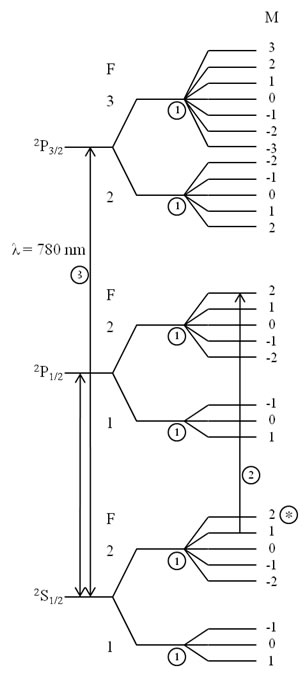
\includegraphics[scale=0.5]{zeeman_splitting.jpg}
    \caption{Schematische Darstellung der Elektronenkonfiguration von Rubidium.\cite{D1}}
    \label{fig:D1}
\end{figure}

\subsection{Quantenzahlen des Atoms}
\label{sec:Quantenzahlen}
Die Energieniveaus eines Atoms lassen sich durch die Hauptquantenzahl $n$, der Bahndrehimpulsquantenzahl $l$
mit $0 \leq l < n$ und der magnetischen Quantenzahl $m$ mit $-l \leq m \leq l$ beschreiben. Rubidium ist ein
Alkalimetall und hat nur ein Valenzelektron, so dass es sich gut durch ein Atom mit einem Elektron annähern lässt.

\subsection{Spin-Bahn-Kopplung}
\label{sec:Spin-Bahn-Kopplung}
Da der Kern im Ruhesystem des Elektrons ein Magnetfeld erzeugt und das Elektron einen Spin hat, spalten sich die
Energieniveaus weiter auf. Dies wird auch Feinstruktur genannt. Die Aufspaltung folgt dem Gesamtdrehimpuls $J$
der sich aus dem Spin und dem Bahndrehimpuls durch $J=L+S$ zusammensetzt. Der Bahndrehimpuls geht von $|L-S|$ bis
$|L+S|$ definiert. Dadurch dass nur ein Valenzelektron vorhanden ist ergibt sich für beide Isotope
$J=S=\frac{1}{2}$.

\subsection{Hyperfeinstruktur}
\label{sec:Hyperfeinstruktur}
Weiterhin gibt es noch eine wesentlich geringere Aufspaltung durch die magnetischen Momente der Kerne. Die
Aufspaltung lässt sich durch die Quantenzahl $F$ beschreiben, die von $|J-I|$ bis $|J+I|$ läuft. Dabei ist
$I$ der Kernspin. Das Isotop $^{85}\symup{Rb}$ hat einen Kernspin von $I=\frac{5}{2}$ und das Isotop
$^{87}\symup{Rb}$ einen Kernspin von $I=\frac{3}{2}$. Mögliche Quantenzahlen sind folglich $F=2$ und $F=3$
für $^{85}\symup{Rb}$ oder $F=1$ und $F=2$ für $^{87}\symup{Rb}$.

\subsection{Zeeman-Effekt}
\label{sec:Zeeman-Effekt}
Eine weiter Aufspaltung lässt sich durch Einschalten eines externen Magnetfels erreichen. Diese Aufspaltung
der Energieniveaus wird durch die Quantenzahl $M_F$ beschrieben, die durch $-F \leq M_F \leq F$ definiert ist.
Dabei entstehen $2F+1$ neue Zeeman-Niveaus mit einer Energiedifferenz von
\begin{equation}
    \label{eq:Ediff}
    E = g_F \mu_B B\,.
\end{equation}
Der enstprechende Land\'e-Faktor bestimmt sich durch
\begin{equation}
    \label{eq:gf}
    g_F = g_J \frac{F(F+1)+J(J+1)-I(I+1)}{2F(F+1)}
\end{equation}
mit
\begin{equation}
    \label{eq:gj}
    g_J = 1 + \frac{J(J+1)+S(S+1)-L(L+1)}{2J(J+1)}\,.
\end{equation}

\subsection{Optisches Pumpen}
\label{sec:OptischesPumpen}
Im Gegensatz zu den inneren Elektronenschalen, die nach dem Pauli-Prinzips besetzt sind, sind die äußeren
Elektronen, unter der Bedingung dass sie das Atom sich im thermischen Gleichgewicht mit der Umgebung
befindet, nach der Boltzmann-Verteilung besetzt. Das Verhältnis der Besetzungszahlen $N_i$ zweier Zustände
ergibt sich durch
\begin{equation}
    \label{eq:Besetzung}
    \frac{N_2}{N_1} = \frac{g_2}{g_1}\frac{exp(\frac{-W_2}{k_B T})}{exp(\frac{-W_1}{k_B T})}\,.
\end{equation}
Dabei ist $T$ die Temperatur, $g_i$ die statistischen Gewichte und $W_i$ die Energien des i-ten Zustands.
Beim optischen Pumpen wird versucht eine Abweichung der Besetzungszahlen zu erzeugen. Wird ausreichend gepumpt
ist eine Inversion der Besetzungszahlen möglich. In diesem Versuch wird zirkular polarisierte $D_1$-Licht
auf das Rubidium eingestrahlt, so dass Elektronen aus dem Grundzustand $^2S_{1/2}$ in den ersten angeregten Zustand
$^2P_{1/2}$ gehoben werden. Die Auswahlregel erlaubt nur $\Delta M = \pm1$ für rechts-/linkspolarisiertes Licht.
Die entsprechenden Übergänge heißen $\sigma^+$ und $\sigma^-$. Fällt linear polarisiertes Licht ein wird von
$\pi$-Übergängen mit $\Delta M = 0$ gesprochen. Im Versuch wird rechtszirkular polarisiertes Licht verwendet.
Nach Anregung in einen höheren Zustand fallen die Elektronen in einen der Grundzustände zurück, so dass auf Dauer
alle Elektronen in einen Zustand gepumpt werden, der nicht weiter angeregt werden kann. Die Emission läuft dabei
spontan oder induziert ab. Bei induzierte Emission wird ein Photon mit der Energie der Energielücke benötigt. Das
angeregte Elektron fällt danach in einen der Grundzustände zurück und emittiert dabei ein identisch zum für die
induzierte Emission benötigtes Photon ab. Die Wahrscheinlichkeit der spontanen Emission hängt von $f^3$ ab.
Aufgrund der Größenordnungen ist dieser Prozess für den Versuch also irrelevant. So bald eine Besetzungsinversion
erreicht ist, lässt sie sich durch ein hochfrequentes RF-Feld wieder aufheben. Die Besetzungsiversion zerfällt,
wenn das RF-Feld genau die Resonanzfrequenz der Zeemanübergänge
\begin{equation}
    \label{eq:Resonanz}
    f = \frac{g_F \mu_B B}{h}
\end{equation}
hat. Die Veränderung des RF-Felds wirkt sich auch auf die Transparenz des Gases und damit auf die Intensität aus.
Ist die Resonanz erreicht, ist das Gas vollständig transparent und ein Dip ist in der Kurve erkennbar. Eine
entsprechende Darstellung des Zusammenhangs ist in \autoref{fig:transparent} zu finden.
\begin{figure}
    \centering
    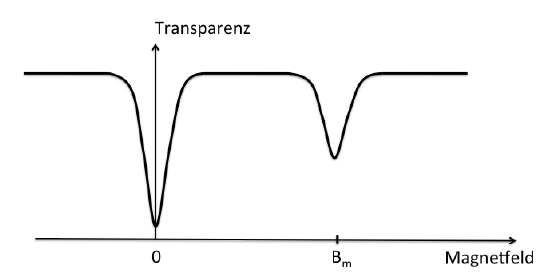
\includegraphics{transparenz.png}
    \caption{Schematische Darstellung der Änderung der Transparenz des Rubidumgases bei sich verändernen
    RF-Feld. \cite{V21}}
    \label{fig:transparent}
\end{figure}